\section{Modelos de Domínio}
Se seguida mostramos os vários diagramas referentes à interligação ds várias entidades de domínio.\\
Na Figura \ref{fig:mdgeral} temos uma visão geral (de nível 0) do modelo de domínio deste projecto. Vemos que existem dois tipos de utilizadores (Normal e Admin)
que acedem ao Visualizador. O Visualizador por si só mostra informação sob a forma de esquemas que podem ser gráficos ou tabelas sobre os ataques.\\

Introduzimos aqui também a noção de plugin, que pode ser visto como um conjunto de contractos que todos os sistemas teêm de cumprir se quiserem desenhar
algum esquema no Visualizador. Portanto podemos ver estes sistemas como webservices que comunicam com o Visualizador para desenhar esquemas.\\

Neste caso, definimos que o produto minimo seria o conjunto de dois sensores um ao nível de rede e outro ao nível do sistema operativo (o Honeypot).
Com estes dois sistemas teremos então cumprido o objectivo principal deste projecto - identificar ataques ao nível de rede e de sistema operativo.\\
O sistema de Sensor de rede usa uma Base de dados para registar o tráfego de rede e os alertas lançados pelo snort. Por outro lado o honeypot
detecta os ataques e regista também na Base de dados estes ataques.

\begin{figure}[!ht]
\centering	
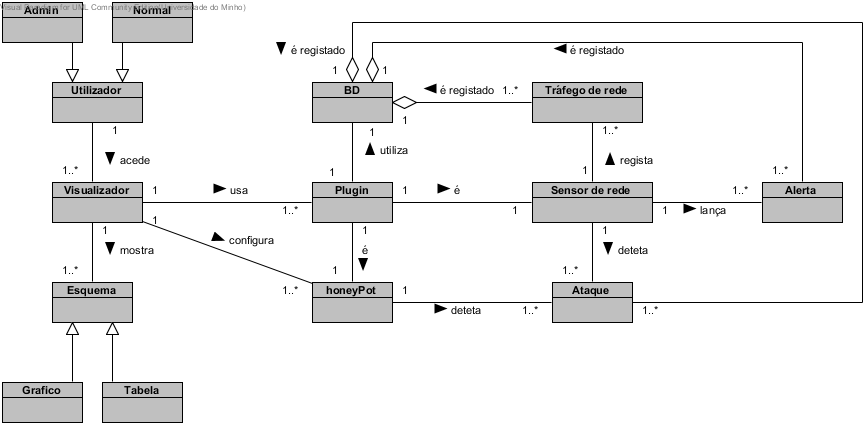
\includegraphics[scale=0.7]{images/ModelosDeDominio/Geral.png}
\caption{Modelo de Domínio Geral}
\label{fig:mdgeral}
\end{figure}

Na Figura \ref{fig:mdhoney} podemos ver o modelo de domínio do Honepot em maior detalhe. É importante referir que este projecto
prevê que o Honeypot esteja a correr numa máquina virtual, porque assim facilita a inspecção. Neste nível de granularidade vemos que existem duas entidades,
uma o sistema operativo Host que é o sistema operativo que corre a máquina virtual e o sistema operativo guest, que é o sistema operativo virtualizado.
O sistema operativo host possui várias instâncias de máquinas virtuais alteradas a que demos o nome de DQEMU, que será um sistema de virtualização
com a capacidade de inspeccionar a actividade do sistema operativo guest. O DQEMU, que supervisiona o guest, quando detectar actividade maliciosa no guest
armazena informação sobre essa actividade na base de dados.\\
De lembrar que o guest possuí propositadamente vulnerabilidades com o intuito de atrair atacantes e assim registar as suas actividades.\\
Este guest pode ter várias personalidades, isto é sistemas operativos reais a correr, entre elas: Linux, Solaris e Windows.

\begin{figure}[!ht]
\centering	
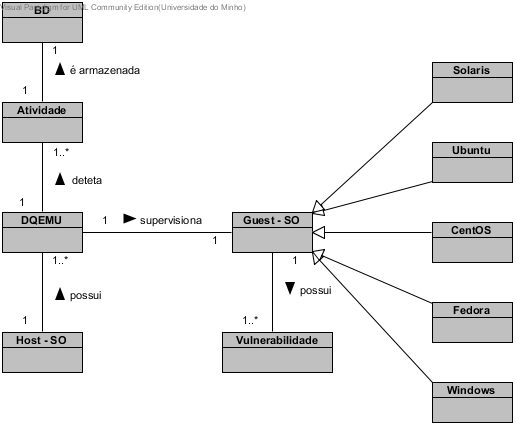
\includegraphics[scale=0.8]{images/ModelosDeDominio/HoneyPot.png}
\caption{Modelo de Domínio HoneyPot}
\label{fig:mdhoney}
\end{figure}

A Figura \ref{fig:mdrede} apresenta o modelo de domínio do sensor de rede, que neste caso será o conjunto de três ferramentas, sendo que uma delas será
construída no ambito deste produto - o Delusion collector daemon. Aqui irá ser necessário utilizar as informações que o tshark e o snort collectam da rede
afim de tirar conslusões sobre a acitivade da rede. Será ainda utilizada uma Base de dados para guardar os alertas do snort e o trágefo de rede, devidamente relacionado
e ainda fazer polling dos alertas do snort.

\begin{figure}[!ht]
\centering	
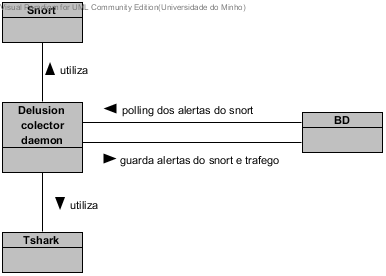
\includegraphics[scale=0.8]{images/ModelosDeDominio/Rede.png}
\caption{Modelo de Domínio Rede}
\label{fig:mdrede}
\end{figure}

A Figura \ref{fig:mdvis} apresenta o modelo de domínio do visualizador onde se pode ver um Filtro que o utilizador usa para restringir a amostragem de
informação (por exemplo pode ser: "mostra-me todos os alertas de ataques das últimas 24 horas"). Este Filtro irá usar a Base de dados para extraír a informação
pretendida e posteriormente esa informação será mostrada em forma de gráfico ou tabela.

\begin{figure}[!ht]
\centering	
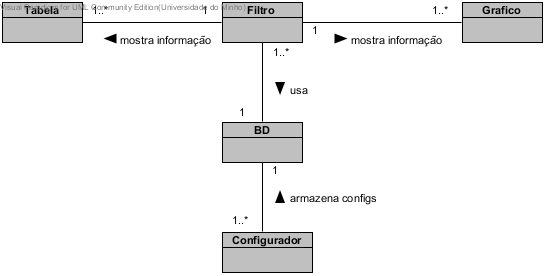
\includegraphics[scale=0.8]{images/ModelosDeDominio/Visualizador.png}
\caption{Modelo de Domínio Visualizador}
\label{fig:mdvis}
\end{figure}
\pagebreak
